\tikzset{every picture/.style={line width=0.75pt}} %set default line width to 0.75pt        

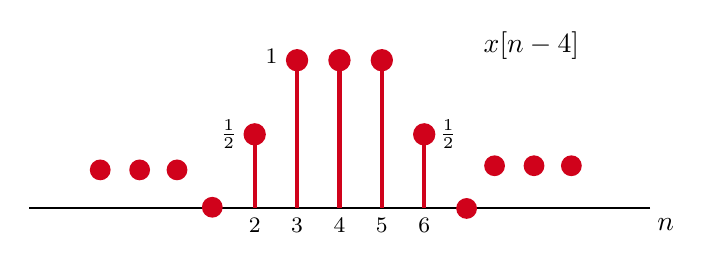
\begin{tikzpicture}[x=0.75pt,y=0.75pt,yscale=-1,xscale=1]
%uncomment if require: \path (0,364); %set diagram left start at 0, and has height of 364

%Straight Lines [id:da06072638558515686] 
\draw    (378.71,168) -- (79.29,168) ;
%Straight Lines [id:da5547538617459793] 
\draw [color={rgb, 255:red, 208; green, 2; blue, 27 }  ,draw opacity=1 ][fill={rgb, 255:red, 208; green, 2; blue, 27 }  ,fill opacity=1 ][line width=1.5]    (229,96.58) -- (229,168) ;
\draw [shift={(229,96.58)}, rotate = 90] [color={rgb, 255:red, 208; green, 2; blue, 27 }  ,draw opacity=1 ][fill={rgb, 255:red, 208; green, 2; blue, 27 }  ,fill opacity=1 ][line width=1.5]      (0, 0) circle [x radius= 4.36, y radius= 4.36]   ;
%Straight Lines [id:da08967735559368817] 
\draw [color={rgb, 255:red, 208; green, 2; blue, 27 }  ,draw opacity=1 ][fill={rgb, 255:red, 208; green, 2; blue, 27 }  ,fill opacity=1 ][line width=1.5]    (249.42,96.58) -- (249.42,168) ;
\draw [shift={(249.42,96.58)}, rotate = 90] [color={rgb, 255:red, 208; green, 2; blue, 27 }  ,draw opacity=1 ][fill={rgb, 255:red, 208; green, 2; blue, 27 }  ,fill opacity=1 ][line width=1.5]      (0, 0) circle [x radius= 4.36, y radius= 4.36]   ;
%Straight Lines [id:da11193473546126165] 
\draw [color={rgb, 255:red, 208; green, 2; blue, 27 }  ,draw opacity=1 ][fill={rgb, 255:red, 208; green, 2; blue, 27 }  ,fill opacity=1 ][line width=1.5]    (208.58,96.58) -- (208.58,168) ;
\draw [shift={(208.58,96.58)}, rotate = 90] [color={rgb, 255:red, 208; green, 2; blue, 27 }  ,draw opacity=1 ][fill={rgb, 255:red, 208; green, 2; blue, 27 }  ,fill opacity=1 ][line width=1.5]      (0, 0) circle [x radius= 4.36, y radius= 4.36]   ;
%Straight Lines [id:da8545689410720038] 
\draw [color={rgb, 255:red, 208; green, 2; blue, 27 }  ,draw opacity=1 ][fill={rgb, 255:red, 208; green, 2; blue, 27 }  ,fill opacity=1 ][line width=1.5]    (269.84,132.29) -- (269.84,167.71) ;
\draw [shift={(269.84,132.29)}, rotate = 90] [color={rgb, 255:red, 208; green, 2; blue, 27 }  ,draw opacity=1 ][fill={rgb, 255:red, 208; green, 2; blue, 27 }  ,fill opacity=1 ][line width=1.5]      (0, 0) circle [x radius= 4.36, y radius= 4.36]   ;
%Straight Lines [id:da9437858155461635] 
\draw [color={rgb, 255:red, 208; green, 2; blue, 27 }  ,draw opacity=1 ][fill={rgb, 255:red, 208; green, 2; blue, 27 }  ,fill opacity=1 ][line width=1.5]    (188.16,132.29) -- (188.16,167.71) ;
\draw [shift={(188.16,132.29)}, rotate = 90] [color={rgb, 255:red, 208; green, 2; blue, 27 }  ,draw opacity=1 ][fill={rgb, 255:red, 208; green, 2; blue, 27 }  ,fill opacity=1 ][line width=1.5]      (0, 0) circle [x radius= 4.36, y radius= 4.36]   ;
%Shape: Circle [id:dp8415745106048833] 
\draw  [color={rgb, 255:red, 208; green, 2; blue, 27 }  ,draw opacity=1 ][fill={rgb, 255:red, 208; green, 2; blue, 27 }  ,fill opacity=1 ] (163.24,167.42) .. controls (163.24,164.94) and (165.25,162.92) .. (167.74,162.92) .. controls (170.22,162.92) and (172.24,164.94) .. (172.24,167.42) .. controls (172.24,169.91) and (170.22,171.92) .. (167.74,171.92) .. controls (165.25,171.92) and (163.24,169.91) .. (163.24,167.42) -- cycle ;
%Shape: Circle [id:dp1924487381459985] 
\draw  [color={rgb, 255:red, 208; green, 2; blue, 27 }  ,draw opacity=1 ][fill={rgb, 255:red, 208; green, 2; blue, 27 }  ,fill opacity=1 ] (285.76,168) .. controls (285.76,165.51) and (287.78,163.5) .. (290.26,163.5) .. controls (292.75,163.5) and (294.76,165.51) .. (294.76,168) .. controls (294.76,170.49) and (292.75,172.5) .. (290.26,172.5) .. controls (287.78,172.5) and (285.76,170.49) .. (285.76,168) -- cycle ;
%Shape: Circle [id:dp9724739272897065] 
\draw  [color={rgb, 255:red, 208; green, 2; blue, 27 }  ,draw opacity=1 ][fill={rgb, 255:red, 208; green, 2; blue, 27 }  ,fill opacity=1 ] (146.24,149.42) .. controls (146.24,146.94) and (148.25,144.92) .. (150.74,144.92) .. controls (153.22,144.92) and (155.24,146.94) .. (155.24,149.42) .. controls (155.24,151.91) and (153.22,153.92) .. (150.74,153.92) .. controls (148.25,153.92) and (146.24,151.91) .. (146.24,149.42) -- cycle ;
%Shape: Circle [id:dp37116477968769124] 
\draw  [color={rgb, 255:red, 208; green, 2; blue, 27 }  ,draw opacity=1 ][fill={rgb, 255:red, 208; green, 2; blue, 27 }  ,fill opacity=1 ] (128.24,149.42) .. controls (128.24,146.94) and (130.25,144.92) .. (132.74,144.92) .. controls (135.22,144.92) and (137.24,146.94) .. (137.24,149.42) .. controls (137.24,151.91) and (135.22,153.92) .. (132.74,153.92) .. controls (130.25,153.92) and (128.24,151.91) .. (128.24,149.42) -- cycle ;
%Shape: Circle [id:dp0005769558109711692] 
\draw  [color={rgb, 255:red, 208; green, 2; blue, 27 }  ,draw opacity=1 ][fill={rgb, 255:red, 208; green, 2; blue, 27 }  ,fill opacity=1 ] (109.24,149.42) .. controls (109.24,146.94) and (111.25,144.92) .. (113.74,144.92) .. controls (116.22,144.92) and (118.24,146.94) .. (118.24,149.42) .. controls (118.24,151.91) and (116.22,153.92) .. (113.74,153.92) .. controls (111.25,153.92) and (109.24,151.91) .. (109.24,149.42) -- cycle ;
%Shape: Circle [id:dp5765900568262574] 
\draw  [color={rgb, 255:red, 208; green, 2; blue, 27 }  ,draw opacity=1 ][fill={rgb, 255:red, 208; green, 2; blue, 27 }  ,fill opacity=1 ] (336.24,147.42) .. controls (336.24,144.94) and (338.25,142.92) .. (340.74,142.92) .. controls (343.22,142.92) and (345.24,144.94) .. (345.24,147.42) .. controls (345.24,149.91) and (343.22,151.92) .. (340.74,151.92) .. controls (338.25,151.92) and (336.24,149.91) .. (336.24,147.42) -- cycle ;
%Shape: Circle [id:dp3702216225275915] 
\draw  [color={rgb, 255:red, 208; green, 2; blue, 27 }  ,draw opacity=1 ][fill={rgb, 255:red, 208; green, 2; blue, 27 }  ,fill opacity=1 ] (318.24,147.42) .. controls (318.24,144.94) and (320.25,142.92) .. (322.74,142.92) .. controls (325.22,142.92) and (327.24,144.94) .. (327.24,147.42) .. controls (327.24,149.91) and (325.22,151.92) .. (322.74,151.92) .. controls (320.25,151.92) and (318.24,149.91) .. (318.24,147.42) -- cycle ;
%Shape: Circle [id:dp5762492676349926] 
\draw  [color={rgb, 255:red, 208; green, 2; blue, 27 }  ,draw opacity=1 ][fill={rgb, 255:red, 208; green, 2; blue, 27 }  ,fill opacity=1 ] (299.24,147.42) .. controls (299.24,144.94) and (301.25,142.92) .. (303.74,142.92) .. controls (306.22,142.92) and (308.24,144.94) .. (308.24,147.42) .. controls (308.24,149.91) and (306.22,151.92) .. (303.74,151.92) .. controls (301.25,151.92) and (299.24,149.91) .. (299.24,147.42) -- cycle ;

% Text Node
\draw (380.71,171.4) node [anchor=north west][inner sep=0.75pt]    {$n$};
% Text Node
\draw (181.16,132.29) node [anchor=east] [inner sep=0.75pt]  [font=\footnotesize]  {$\frac{1}{2}$};
% Text Node
\draw (275.84,132.29) node [anchor=west] [inner sep=0.75pt]  [font=\footnotesize]  {$\frac{1}{2}$};
% Text Node
\draw (200.58,94.58) node [anchor=east] [inner sep=0.75pt]  [font=\footnotesize]  {$1$};
% Text Node
\draw (188.16,171.11) node [anchor=north] [inner sep=0.75pt]  [font=\footnotesize]  {$2$};
% Text Node
\draw (208.58,171.4) node [anchor=north] [inner sep=0.75pt]  [font=\footnotesize]  {$3$};
% Text Node
\draw (229,171.4) node [anchor=north] [inner sep=0.75pt]  [font=\footnotesize]  {$4$};
% Text Node
\draw (249.42,171.4) node [anchor=north] [inner sep=0.75pt]  [font=\footnotesize]  {$5$};
% Text Node
\draw (269.84,171.11) node [anchor=north] [inner sep=0.75pt]  [font=\footnotesize]  {$6$};
% Text Node
\draw (297,81.4) node [anchor=north west][inner sep=0.75pt]    {$x[ n-4]$};


\end{tikzpicture}
